\documentclass[11pt]{article}
\usepackage[utf8]{inputenc}
\usepackage[english]{babel}
\usepackage{graphicx}
\usepackage{blindtext}
\usepackage{listings}
\usepackage{hyperref}
\usepackage{longtable}
%Gummi|065|=)
\title{\textbf{Automatas celulares}}
\author{Juan Carlos Olivier Jasso\\}
\date{11 Abril 2016} 
\begin{document}

\maketitle
\tableofcontents
\clearpage

\section{Introduccion}

\emph{Modelo matematico para un sistema dinámico que evoluciona en pasos discretos.} Es decir, es un modelo matemático para sistemas que soportan cambios; además, estos cambios se suceden cada tiempos constantes, razón por la cual, se usa una escala de enteros. \\
 	
La idea de la creacion de los automatas celulares nacion en la decada de 1940 en donde John Von Neumann, intentaba la creacion de un sistema que pudiera autoreplicarse o extenderse de forma autonoma, mediante un modelo matematico, aplicados en una red rectangular. Contenian celulas las cuales asemejaban al proceso de vida en donde crecian, se reproducian y morian conforme pasaba el tiempo, Tienen diferentes valores y comportamientos entre si.\\

Se define Lattice,es una cuardicula de dimension N e infinitamente extendida. Dentro de cada una de las celdas en la cuadricula se encuentra una \emph{"Celula"}. Cada celula toma un valor de un conjunto finito de estados \emph{k}, el ciclo de vida de la celula y su evolucion no dependera solo de ella, si no, tambien de su entrono, los cuales determinaran sus condiciones de vida. Para determinar su evolucion, la funcion de reticula, se aplica a cada una de la celulas dentro de la \emph{lattice}, toma todos los valores de la celda y sus alrededores-, asi podra determinar los nuevos valores de cada celula.

\newpage

\section{Automatas celulares unidimensionales}

Consiste en una sola fila de células a los que se aplica un principio de vecindad básico de dos vecinos por célula y a los que igualmente se pueden aplicar las diversas condiciones de frontera que hemos nombrado anteriormente

\begin{figure}[htp]
\centering
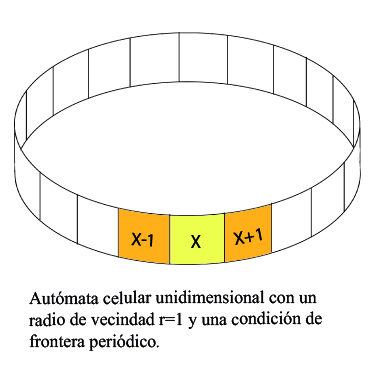
\includegraphics[width=6.5cm]{01.jpg}
\label{fig:lion}
\end{figure}

Como ejemplo, podemos tomar un autómata celular unidimensional con un radio de vecindad r=1, dos estados (0 y 1) y una condicion de frontera de tipo periódico, como el que se muestra en la imagen. Usaremos para este caso un tamaño de diez células y unas funciones de transición basadas en lo siguiente: 
\begin{itemize}
  \item Si ambos vecinos de la célula tienen el mismo estado, el estado de la célula a la que se aplica la funcion cambiará.
  \item Si ambos vecinos de la célula tienen distinto estado, el estado de la célula a la que se aplica se mantendrá igual.
\end{itemize}

\clearpage

Stephen Wolfram clasificó el comportamiento de los automatas celulares unidimensionales. Según Wolfram, todo automata celular pertenece a una de las siguientes clases:

\begin{itemize}
  \item Clase I. La evolución lleva a una configuración estable y homogénea, es decir, todas las células terminan por llegar al mismo valor.
  \item Clase II. La evolución lleva a un conjunto de estructuras simples que son estables o periódicas.
  \item Clase III. La evolución lleva a un patrón caótico1.
  \item Clase IV. La evolución lleva a estructuras aisladas que muestran un comportamiento complejo (es decir, ni completamente caótico, ni completamente ordenado, sino en la línea entre uno y otro, este suele ser el tipo de comportamiento más interesante que un sistema dinámico puede presentar).
\end{itemize}

\section{Autómatas celulares bidimensionales}

    Un autómata celular finito de 2 estados es la simulación más simplificada posible de una célula viva sobre un tejido. Representa una unidad de interacción que tan solo puede presentar 2 estados (activo e inerte, encendido y apagado, vivo o muerto, o como quieran denominarse). A pesar de su simplicidad inicial permite simular la evolución de sistemas complejos y analizar pautas tales como el comportamiento emergente.
    Un nuevo nivel de complejidad consiste en trabajar con un autómata celular de 2 estados, situado en un universo plano (de 2 dimensiones) ilimitado (toroidal, cerrado circularmente en sus dos direcciones).\\
    
    
El autómata posee solo 2 estados, representados por dos imagenes distintas. El estado evolutivo del autómata dependerá de su estado actual y el de su entorno (sus 8 células vecinas, derecha, izquierda, arriba, abajo y las cuatro esquinas).El universo es cerrado e ilimitado (toroidal), de forma que las últimas celdas de la derecha están unidas (interactuan) con las primeras de la izquierda y viceversa, al igual que las de la línea inferior lo hacen con la primera y viceversa. La evolución es discreta y simultánea para todos los componentes (células) del universo. Cada generación surgirá de golpe reemplazando completamente a la anterior.

\clearpage

Las reglas para una evolucion son las siguientes:
\begin{itemize}
\item Una célula se inactiva (o permanece inactiva) si posee menos de 2 o más de 3s vecinas activas (muerte).
\item Una célula mantiene su estado, sea este cual fuera, si tiene tan solo 2 células vecinas activas (conservación).
\item Una célula cobra actividad (o permanece activa si ya lo estaba) cuando la rodean 3 células activas (nacimiento).
\end{itemize}

\begin{figure}[htp]
\centering
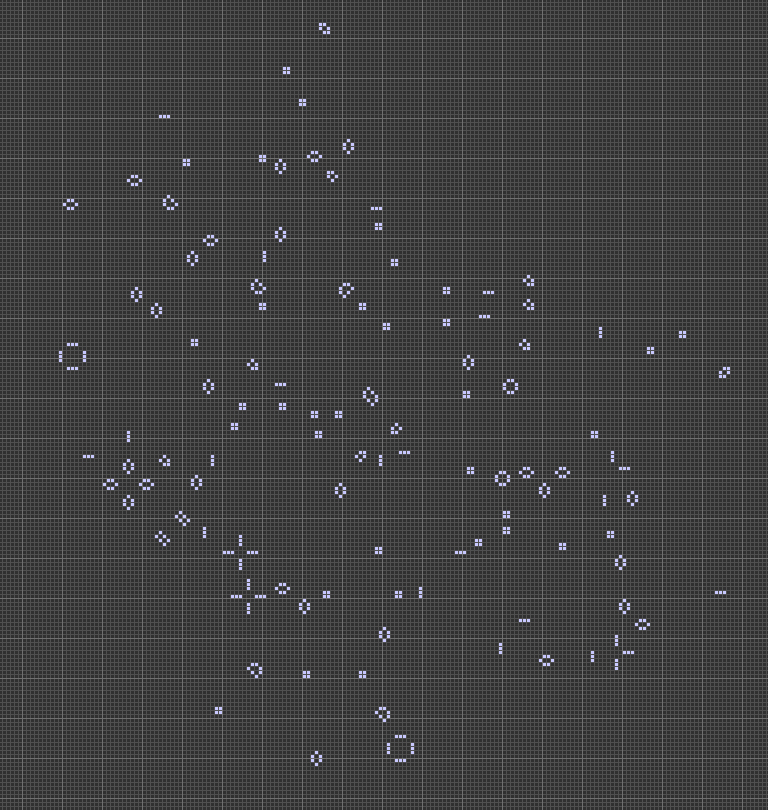
\includegraphics[width=6.5cm]{8.jpg}
\label{fig:lion}
\end{figure}

\clearpage

\section{Autómatas celulares tridimensionales}

Ampliamente estudiados por Carter Bays, los automatas celulares de tres dimensiones se enfocan principalmente para encontrar una regla de evolución en tres dimensiones que sea la sucesora del Juego de la Vida en el espacio tridimensional, muchos de sus resultados son de tipo cuantitativo, basados principalmente en la simulación de varias reglas de evolución en pequeños espacios tridimensionales para encontrar estructuras que sean similares al Juego.La aplicación de estos autómatas celulares se centra en el estudio en campos estadísticos.\\

Son automatas celulares que se desarrollan en un ámbito de Z x Z x Z, que usan el principio de vecindad de Moore a nivel tridimensional. Esto implica que la función de transición ha de tener en cuenta el estado de veintiseis células vecinas además del estado de la célula en cuestión.\\

Los automatas celulares tridimensionales pueden seguir los mismos principios que los anteriores, aunque dado el incremento de la complejidad de los calculos y el procesamiento, su puesta en práctica no es simple. Sin embargo, y puesto que se pueden considerar automatas celulares tridimensionales con las mismas variables de tipo frontera en el ámbito teórico, se debe considerar que la representacion de los automatas celulares tridimensionales considerando una frontera periódica es en forma de toroide. 

\begin{figure}[htp]
\centering
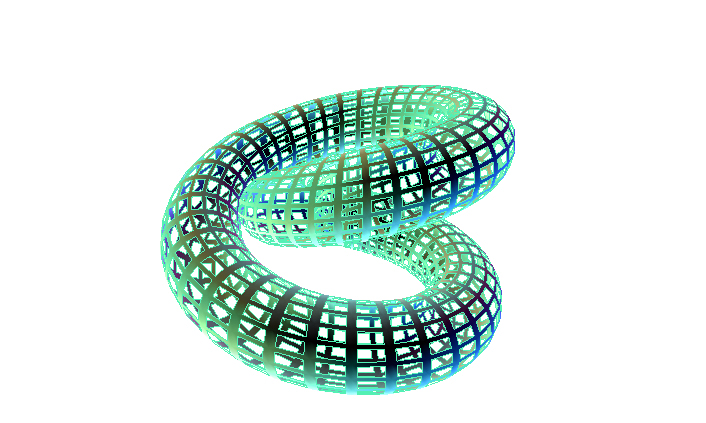
\includegraphics[width=8.5	cm]{10.jpg}
\label{fig:lion}
\end{figure}

\clearpage

\section{Codigo twocellular}

\lstinputlisting{twocellular.cpp}

\section{celullar automata}
\begin{verbatim}

	# include <cstdlib>
	# include <iostream>
	# include <ctime>

	using namespace std;

	int main ( );
	void timestamp ( );

	int main ( )
	{
	  int i;
	  int j;
	  int n;
	  int step_num;
	  char *x;
	  char *x_old;

	  timestamp ( );
	  cout << "\n";
	  cout << "CELLULAR_AUTOMATON:\n";
	  cout << "  C++ version.\n";

	  n = 80; // cantidad de pasos
	  step_num = 80;

	  x = new char[n+2]; //se crea en memorial la ubicacion de la celula actual
	  x_old = new char[n+2]; //se crea en memorial la ubicacion de la celula muerta

	  for ( i = 0; i <= n + 1; i++ ) // inicialicacion de la lattice
	  {
	    x[i] = ' ';
	  }
	  x[40] = '*'; //en la ultima ubicacion de ponte la primera celular

	  for ( i = 1; i <= n; i++ )
	  {
	    cout << x[i];  // se imprime la primera fila
	  }
	  cout << "\n";

	  for ( j = 1; j <= step_num; j++ ) // se guarda la lattice anterior
	  {
	    for ( i = 0; i < n + 2; i++ )
	    {
	      x_old[i] = x[i];
	    }
	    for ( i = 1; i <= n; i++ )
	    {
	//
	//  The transformation rules are:
	//
	//  111  110  101  100  011  010  001  000
	//   |    |    |    |    |    |    |    |
	//   0    0    0    1    1    1    1    0
	//
	//  which means this rule has binary code 00011110 = 16 + 8 + 4 + 2 = 30

	//  Determina si vive o muere depende de lo que se tenga en la lattice donde se guarda lo anterior

	      if ( ( x_old[i-1] == ' ' && x_old[i] == ' ' && x_old[i+1] == '*' ) ||
	           ( x_old[i-1] == ' ' && x_old[i] == '*' && x_old[i+1] == ' ' ) ||
	           ( x_old[i-1] == ' ' && x_old[i] == '*' && x_old[i+1] == '*' ) ||
	           ( x_old[i-1] == '*' && x_old[i] == ' ' && x_old[i+1] == ' ' ) )
	      {
	        x[i] = '*';
	      }
	      else
	      {
	        x[i] = ' ';
	      }
	    }
	//
	// Hacer cumplir las condiciones de contorno periódicas .
	//
	    x[0] = x[n];
	    x[n+1] = x[1];

	    for ( i = 1; i <= n; i++ )
	    {
	      cout << x[i];
	    }
	    cout << "\n";
	  }
	//
	//  Se libera la memoria por el stackoverflow
	//
	  delete [] x;
	  delete [] x_old;
	//
	//  Terminate.
	//
	  cout << "\n";
	  cout << "CELLULAR_AUTOMATON:\n";
	  cout << "  Normal end of execution.\n";
	  cout << "\n";
	  timestamp ( );

	  return 0;
	}
	//****************************************************************************80

	void timestamp ( )

/*
	Imprime el tiempo en el cual se corrio el programa

	*/
	{
	# define TIME_SIZE 40

	  static char time_buffer[TIME_SIZE];
	  const struct std::tm *tm_ptr;
	  size_t len;
	  std::time_t now;

	  now = std::time ( NULL );
	  tm_ptr = std::localtime ( &now );

	  len = std::strftime ( time_buffer, TIME_SIZE, "%d %B %Y %I:%M:%S %p", tm_ptr );

	  std::cout << time_buffer << "\n";

	  return;
	# undef TIME_SIZE
	}

\end{verbatim}



\end{document}
